\chapter{Revisión de la literatura}
La selección de características es un problema cuya popularidad ha ido en aumento con el paso de los años. No es algo casual, pues la cantidad de datos recogidos para tareas de aprendizaje automático y áreas derivadas, como el aprendizaje profundo, ha ido en aumento de manera casi exponencial.\\[6pt]
En este trabajo, se lleva a cabo una investigación y análisis comparativo entre varios métodos
de la familia \textbf{wrapper} o métodos de envoltura. Existen multitud de estrategias~\cite{miao_survey_2016}
que intentan dar solución a este problema. Los métodos de búsqueda más famosos son los de filtrado
(\textbf{filter}), los cuáles seleccionan las características más discriminativas según la naturaleza de los datos~\cite{miao_survey_2016}.
Por lo general, estos métodos realizan la selección de características antes de las tareas de clasificación y
agrupamiento. Ejemplos de algoritmos de filtrado son \textit{relieF}~\cite{kira_practical_1992} o F-statistic~\cite{ding_minimum_2005}.\\[6pt]
Los métodos \textbf{wrapper}, en cambio, utilizan el algoritmo de aprendizaje usado post-procesamiento
para evaluar las características y seleccionar así las más útiles~\cite{miao_survey_2016}.\\[6pt]
Los algoritmos clasificatorios de aprendizaje utilizados en este trabajo son \textit{SVM}~\cite{cortes_support-vector_1995}
y \textit{kNN}~\cite{fix_discriminatory_1989,cover_nearest_1967}, siendo las máquinas de vectores de
soporte un método robusto y eficiente y los vecinos más cercanos un método simple, interpretable
y muy eficaz. Se analizará el resultado entre ambos clasificadores entre otros muchos análisis comparativos.

\begin{figure}[htp]
  \begin{center}
    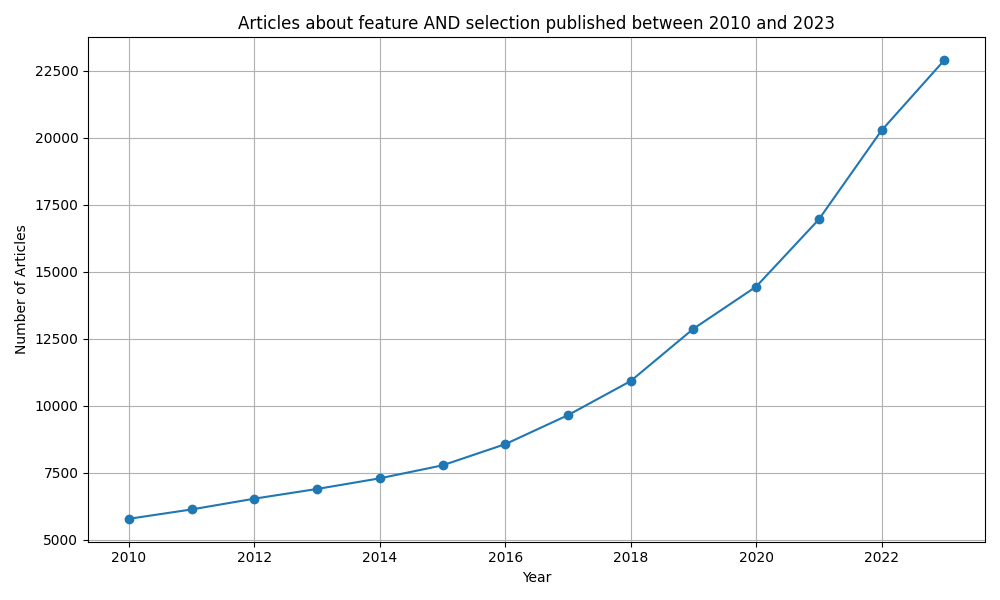
\includegraphics[width=1\textwidth]{imagenes/scopus_chart.png}
  \end{center}
  \caption[Popularidad de feature selection sobre los años]{En esta figura se muestra el número de artículos publicados relacionados con la selección de características. Se ha usado el buscador Scopus para estos resultados.}
  \label{fig:pop_fs}
\end{figure}

\begin{figure}[htp]
  \begin{center}
    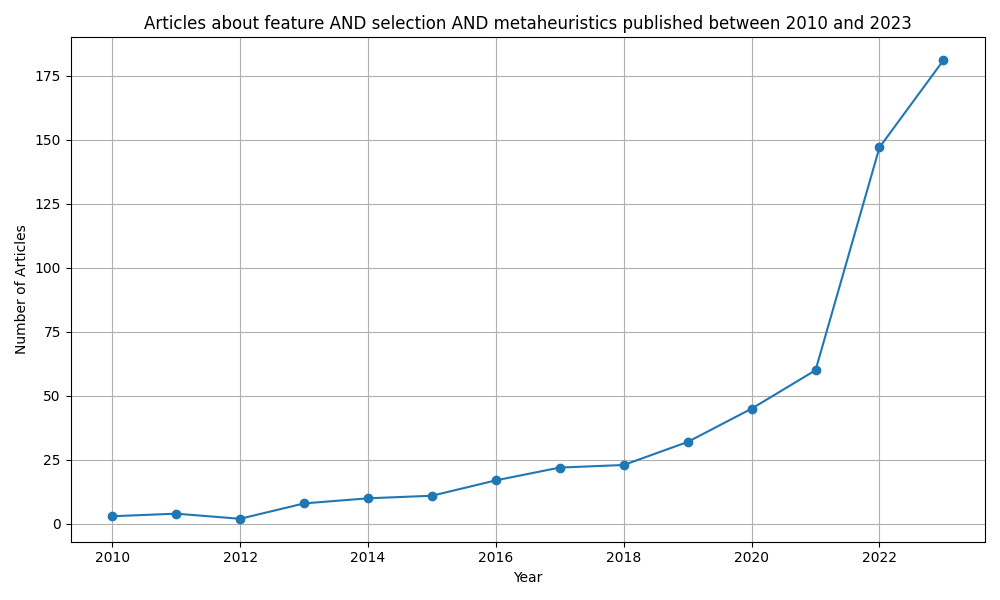
\includegraphics[width=1\textwidth]{imagenes/scopus_chart2.png}
  \end{center}
  \caption[Popularidad de feature selection + metaheuristics sobre los años]{De igual forma que en la figura \ref{fig:pop_fs} las mateheuristicas han ido muy ligadas a la resolución de este problema. Se ha usado el buscador Scopus para estos resultados.}
  \label{fig:pop_fs2}
\end{figure}

Se puede observar en \ref{fig:pop_fs} la creciente popularidad de los métodos de selección de características en el buscador de \textbf{Scopus}. La tendencia parece indicar que la tendencia científica puede incluso crecer aún más alrededor del problema de selección de características. Y es que pese a los grandes avances en \textit{hardware}, parte del techo con el que se topan los algoritmos de aprendizaje sigue siendo los enormes tiempos de entrenamiento.
También ha de mencionarse la tendencia, prácticamente igual en cuanto a escala de crecimiento, en la popularidad sobre los años del problema de selección de características, pero abordado con técnicas metaheurísticas \ref{fig:pop_fs2}.

Y es que las metaheurísticas son algoritmos muy convenientes en la resolución de este tipo de problemas. Los algoritmos analíticos pueden enfrentar dificultades cuando el conjunto de datos tiene un número muy elevado de características, debido a que la cantidad de combinaciones posibles puede hacer que el problema sea inabordable en términos computacionales. Debido a ello, se suelen utilizar algoritmos más rápidos cuya solución no es óptima en términos globales, pero si suficientemente buena.\\[6pt]
Muchos algoritmos metaheurísticos han sido propuestos a lo largo de los años. Se han escogido los más destacables en cuanto a resultados y más mencionados entre todos ellos, dando una selección de algoritmos metaheurísticos modernos de, en principio, muy alta calidad. No solo son seleccionados algoritmos modernos, sino que también se han escogido una serie de algoritmos más ``clásicos'', pero cuya aplicación es más extendida y con resultados que, de forma empírica, han demostrado ser más que buenos a lo largo de décadas de uso.

\begin{table}[htp]
  \parbox{.45\linewidth}{
    \centering
    \begin{tabular}{l}
      \hline
      Algoritmos                         \\ \hline
      GWO~\cite{mirjalili_grey_2014}     \\
      FA~\cite{yang_chapter_2014}        \\
      GOA~\cite{saremi_grasshopper_2017} \\
      WOA~\cite{mirjalili_whale_2016}    \\
      DA~\cite{mirjalili_dragonfly_2016} \\
      CS~\cite{yang_cuckoo_2010}         \\
      BA~\cite{yang_new_2010}            \\
      \hline
    \end{tabular}
    \caption{Algoritmos modernos}
  }
  \hfill
  \parbox{.45\linewidth}{
    \centering
    \begin{tabular}{l}
      \hline
      Algoritmos                        \\ \hline
      PSO~\cite{kennedy_particle_1995}  \\
      GA~\cite{Holland:1975}            \\
      ACO~\cite{dorigo_ant_1999}        \\
      DE~\cite{storn_differential_1997} \\
      ABCO~\cite{karaboga_idea_nodate}  \\
      \hline
    \end{tabular}
    \caption{Algoritmos clásicos}
  }
\end{table}

Los algoritmos usados en este proyecto pertenecen todos a la sub-categoría conocida como algoritmos poblacionales, esto es, algoritmos que parten de un conjunto de soluciones inicializadas de forma aleatoria y representadas en forma de vectores llamadas población. Este tipo de algoritmos ``evolucionan'' durante un número de generaciones hasta alcanzar un máximo número de generación o alcanzar un miembro de la población cuya solución sea lo suficientemente buena~\cite{simon2013evolutionary}.

\section{Introducción a los primeros algoritmos poblacionales}

Uno de los primeros algoritmos basados en poblaciones y evolutivos es el algoritmo genético. Los \textit{algoritmos genéticos} o \textbf{GAs} ganaron popularidad en los años $70$, particularmente en $1975$ con el libro de John Holland~\cite{Holland:1975}. Este tipo de metaheurísticas son diseñadas basándose en la selección natural. Un conjunto de fenotipos (soluciones) son evolucionadas durante generaciones para emular el cruce entre especies (cruce de soluciones mediante un intercambio común de cromosomas) dando lugar a nuevos individuos con características de ambos padres. Poco a poco este tipo de algoritmos fueron desarrollando nuevas características y aunque en un principio fueron diseñados para resolver problemas discretos, también tienen versiones que optimizan problemas continuos~\cite{eiben2015}.\\[6pt]
Uno de los primeros algoritmos metaheurísticos basados en poblaciones es el \textit{sistema de hormigas} de Dorigo, que fue presentado en $1991$~\cite{as}. Esta metaheurística fue aplicada a la resolución del problema del vendedor ambulante con resultados muy prometedores, pues resolvía el problema de forma muy eficiente con una solución sub-óptima, pero suficientemente buena. A partir de este punto, surgieron numerosas mejoras y versiones de los algoritmos basados en colonias de hormigas.\\[6pt]
Más tarde se presentó el conocido algoritmo de \textit{optimización por enjambre de partículas}, nombrado como \textbf{PSO} por sus siglas en inglés y presentado por Kennedy y Eberhart en $1995$~\cite{kennedy_particle_1995}. El algoritmo \textbf{PSO} surgió a partir de la observación del comportamiento social de las aves y peces. La idea principal del \textbf{PSO} es que cada solución candidata (o ``partícula'') en el espacio de búsqueda se mueve a través del espacio en función de su propia mejor posición conocida y la mejor posición conocida de cualquier partícula en el enjambre, en lugar de depender de operadores de búsqueda convencionales. El algoritmo comenzaba con un conjunto de soluciones candidatas aleatorias, denominadas partículas, que procedían a moverse a través del espacio de búsqueda para encontrar la solución óptima. Cada partícula tenía una posición y una velocidad asociadas.\\[6pt]
En $1999$ se presentó el conocido \textbf{ACO} u \textit{optimización de colonia de hormigas}~\cite{dorigo_ant_1999}. Este algoritmo refinada la fórmula anteriormente usada en \textbf{AS} usando un grafo como representación del conjunto de soluciones, la actualización y rastro de feromona como heurística principal para escoger el camino en el grafo y una codificación discreta de las características.\\[6pt]
La \textit{evolución diferencial} fue un algoritmo de optimización propuesto por primera vez por Rainer Storn y Kenneth Price en el año $1997$~\cite{storn_differential_1997}. Surgió como una alternativa a los algoritmos genéticos existentes en ese momento, ya que se inspiraba en su diseño, pero siendo inicialmente diseñado para resolver problemas continuos, a diferencia de los \textbf{GAs}.\\[6pt]
La idea detrás de la evolución diferencial se basaba en la exploración de un espacio de búsqueda mediante la manipulación de vectores de parámetros. A diferencia de los \textit{GAs}, que utilizaban operadores genéticos como la cruza y la mutación, la \textbf{DE} se centraba principalmente en la mutación basada en la diferencia entre vectores de la población. Inicialmente, el algoritmo atrajo la atención debido a su simplicidad y eficiencia en la optimización de funciones complejas en espacios de búsqueda continuos.\\[6pt]
El algoritmo de optimización basado en colonias de abejas es considerado otro gran clásico de las metaheurísticas poblacionales bio-inspiradas, pese a ello, es el más nuevo de los ya mencionados. El algoritmo de colonias de abejas artificiales o \textbf{ABCO} fue propuesto por primera vez por Dervis Karaboga en $2005$~\cite{karaboga_idea_nodate}. Surgió como una técnica inspirada en el comportamiento de las colonias de abejas para resolver problemas de optimización y se basaba en imitar el comportamiento de las abejas en la búsqueda de alimentos. En la naturaleza, las abejas utilizan la danza de reclutamiento para comunicar la ubicación de las fuentes de alimento a otras abejas en la colmena. Karaboga adaptó este proceso en un algoritmo de optimización que utiliza abejas artificiales para explorar y explotar un espacio de búsqueda.

\section{Propuestas metaheurísticas modernas}
Con el paso de los años se han ido refinando y probando nuevos tipos de algoritmos. Nuevas inspiraciones, basadas en el comportamiento animal, en teoría social, en teoría física o matemática. También se han creado nuevas versiones de algoritmos clásicos para resolver ciertos problemas que el algoritmo tenía de base o abordar otros nuevos. De cualquier manera, el número de nuevas metaheurísticas no ha dejado de crecer desde su origen, pues sus usos son muy extensos. Desde la selección de características hasta métodos de búsqueda de hiper-parámetros muy eficientes y con muy buenos resultados~\cite{jaderberg2017population}.

\begin{figure}[htp]
  \begin{center}
    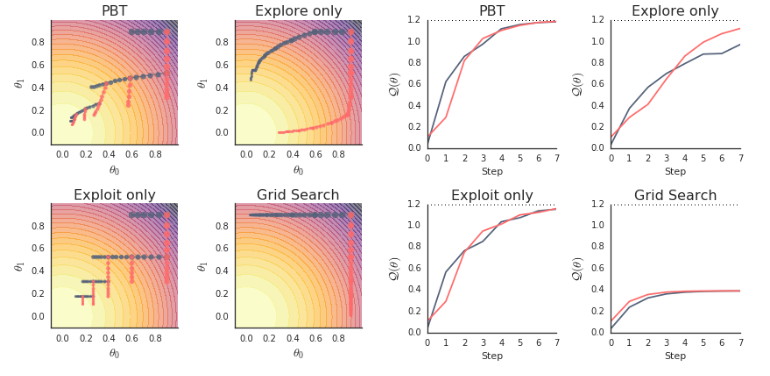
\includegraphics[width=1\textwidth]{imagenes/pbt.png}
  \end{center}
  \caption[PBT en Redes Neuronales]{En esta figura se muestra varios métodos usados en la búsqueda de hiper-parámetros frente al método basado en poblaciones \textbf{PBT}. La zona más blanca representa el mínimo, ya que se trata de minimizar un error de pérdida a la vez que se maximiza una métrica concreta. Population-based training (\textbf{PBT}) es una técnica en el ámbito del aprendizaje automático y el entrenamiento de modelos que combina conceptos de algoritmos genéticos y métodos de ajuste de hiper-parámetros para mejorar el rendimiento y la eficiencia del entrenamiento de modelos.~\cite{jaderberg2017population}}
\end{figure}

Dada una exhaustiva investigación, que incluye múltiples búsquedas en los últimos años en el motor de búsqueda de Scopus y una extensa lectura de varios estudios (``surveys'')~\cite{dokeroglu_comprehensive_2022, agrawal_metaheuristic_2021, boussaid_survey_2013} enfocados en metaheurísticas aplicadas a la \textbf{selección de características} se ha hecho una lista de los más usados, citados y con mejores resultados.

\begin{figure}[htp]
  \centering
  \begin{subfigure}[b]{0.45\textwidth}
    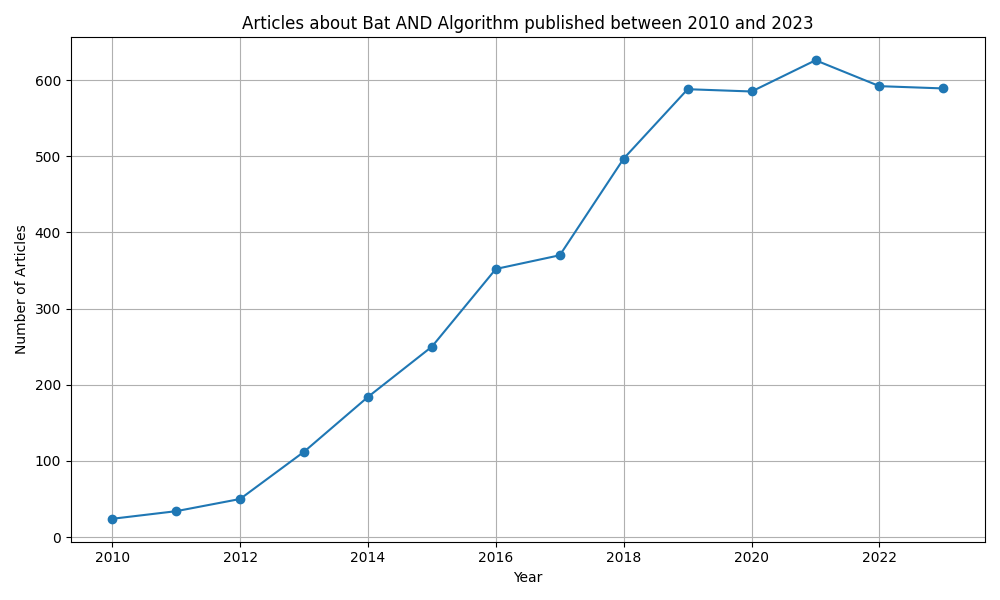
\includegraphics[width=\textwidth]{imagenes/scopus_chart_Bat_Algorithm.png}
    \caption{BA}
    \label{fig:bat_algorithm}
  \end{subfigure}
  \begin{subfigure}[b]{0.45\textwidth}
    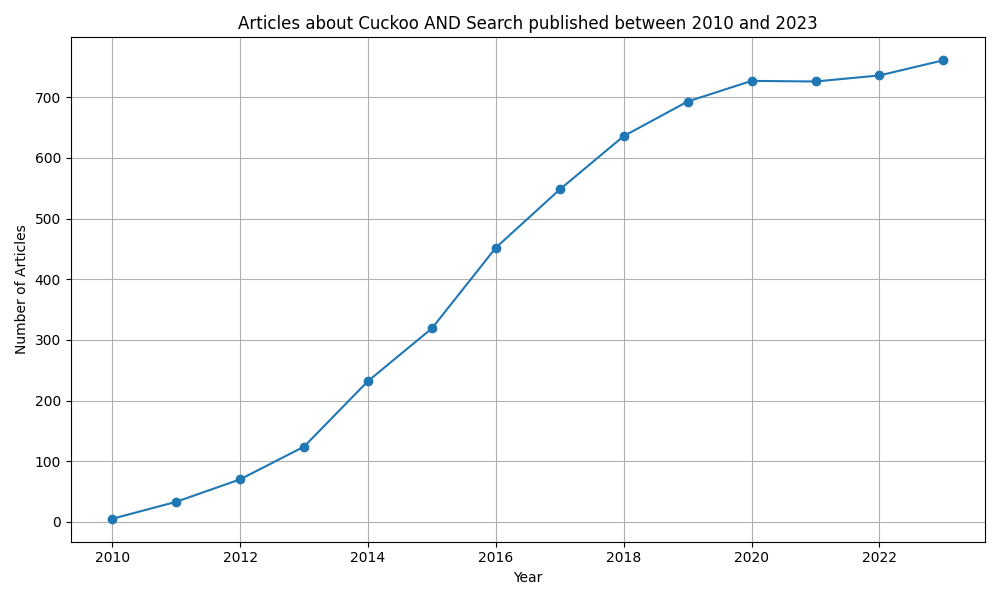
\includegraphics[width=\textwidth]{imagenes/scopus_chart_Cuckoo_Search.png}
    \caption{CS}
    \label{fig:cuckoo_search}
  \end{subfigure}
  \begin{subfigure}[b]{0.45\textwidth}
    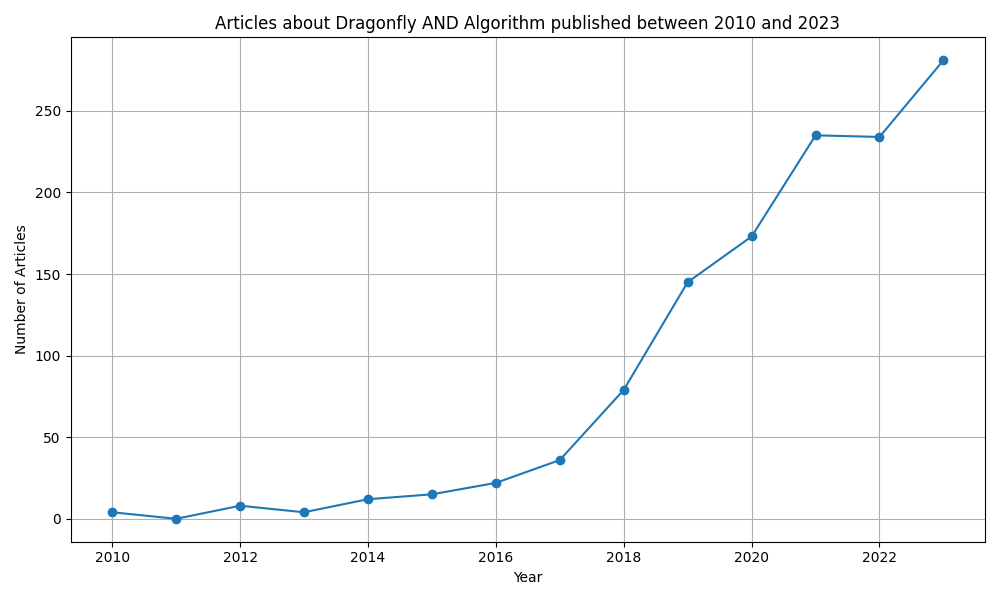
\includegraphics[width=\textwidth]{imagenes/scopus_chart_Dragonfly_Algorithm.png}
    \caption{DA}
    \label{fig:dragonfly_algorithm}
  \end{subfigure}
  \vspace{0.5cm}
  \begin{subfigure}[b]{0.45\textwidth}
    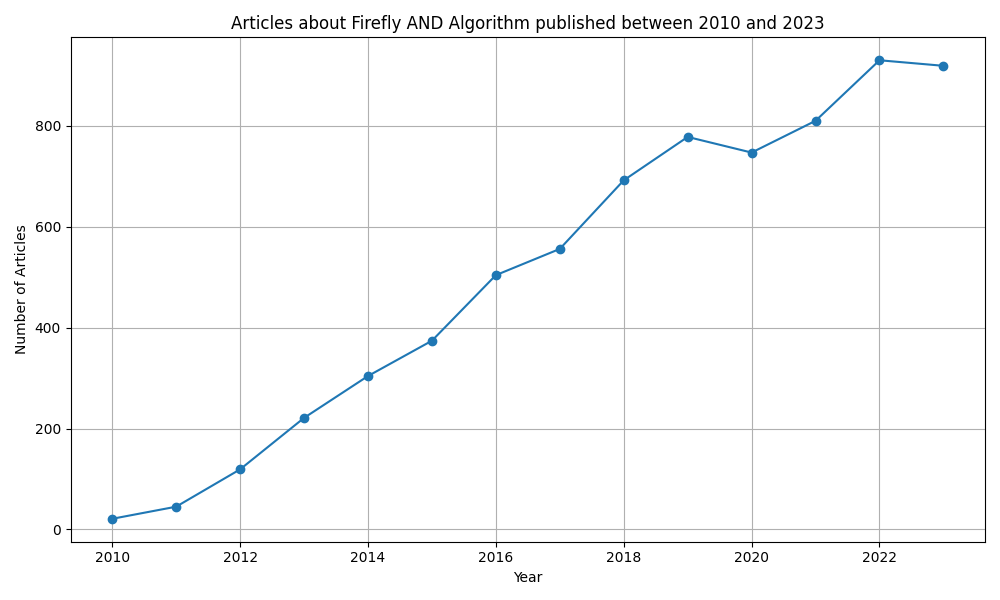
\includegraphics[width=\textwidth]{imagenes/scopus_chart_Firefly_Algorithm.png}
    \caption{FA}
    \label{fig:firefly_algorithm}
  \end{subfigure}
  \begin{subfigure}[b]{0.45\textwidth}
    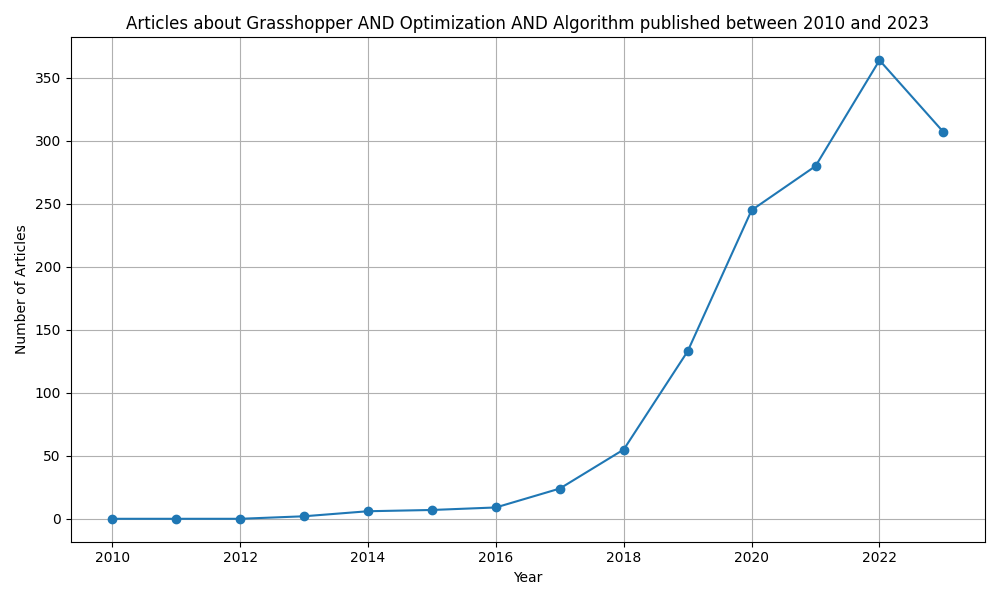
\includegraphics[width=\textwidth]{imagenes/scopus_chart_Grasshopper_Optimization_Algorithm.png}
    \caption{GOA}
    \label{fig:grasshopper_algorithm}
  \end{subfigure}
  \begin{subfigure}[b]{0.45\textwidth}
    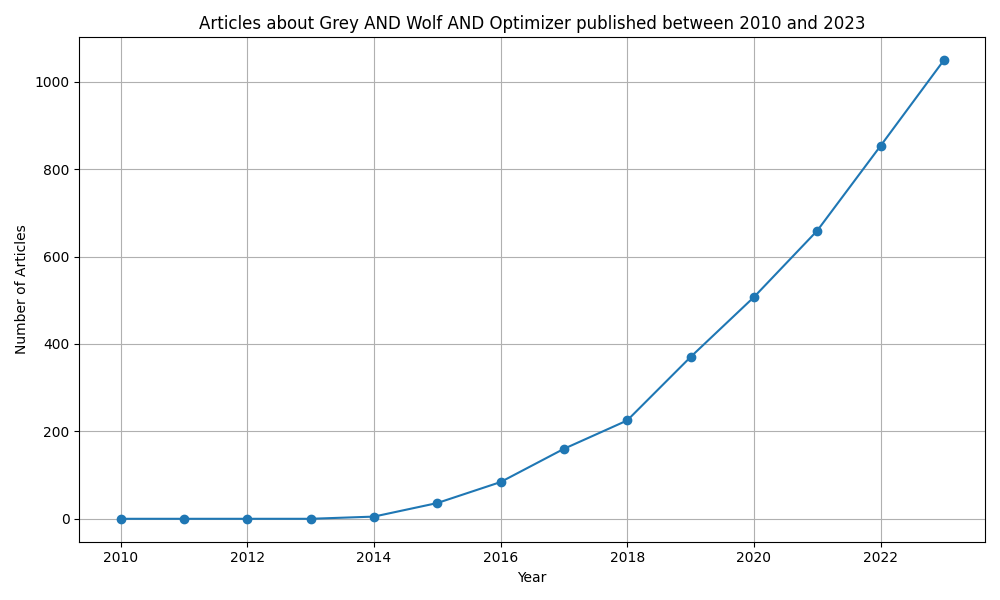
\includegraphics[width=\textwidth]{imagenes/scopus_chart_Grey_Wolf_Optimizer.png}
    \caption{GWO}
    \label{fig:grey_wolf_optimizer}
  \end{subfigure}
  \vspace{0.5cm}
  \begin{subfigure}[b]{0.45\textwidth}
    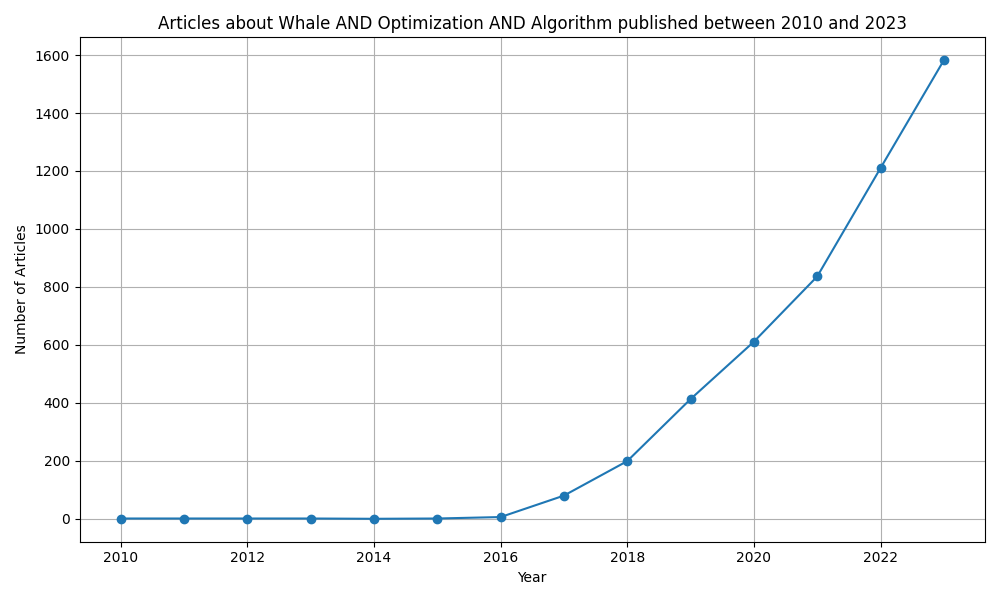
\includegraphics[width=\textwidth]{imagenes/scopus_chart_Whale_Optimization_Algorithm.png}
    \caption{WOA}
    \label{fig:whale_optimization_algorithm}
  \end{subfigure}
  \caption[Popularidad metaheurísticas modernas]{Número de búsquedas en Scopus de los diferentes algoritmos metaheurísticos seleccionados. Se puede ver una clara tendencia alcista en la popularidad de estos pese a su relativa novedad en el campo de la optimización.}
  \label{fig:conjunto_imagenes}
\end{figure}

El más ``antiguo'', dentro de la novedad, de los siete algoritmos aquí citados, es el de la \textit{búsqueda cuco} o \textbf{CS} dadas sus siglas en inglés. Este algoritmo fue presentado a finales de $2009$. En el artículo original~\cite{yang_cuckoo_2010} comparaba su rendimiento con un clásico ya mencionado en este capítulo, el \textbf{PSO}.\\[6pt]
Esto no es novedad, todos los algoritmos más recientes hacen gala de sus buenos resultados en comparación a algoritmos clásicos como son el \textbf{ABCO}, \textbf{DE} o \textbf{PSO} entre otros muchos.\\[6pt]
La búsqueda cuco se inspiraba en el comportamiento parasitario de los pájaros de cuyo nombre de apropia. Estos colocan sus huevos en los nidos de otras aves y además retiran los huevos ajenos para incrementar las posibilidades de incubación de los suyos. Esto pequeña premisa se simula matemáticamente por los agentes de la población y se combina con el uso de funciones que simulan vuelos Lévy (pues se ha observado que el patrón de vuelos de muchas aves e insectos tienden a encajar en ese tipo de distribución~\cite{GUY2008585}).\\[6pt]
El \textit{algoritmo de los lobos grises} o \textbf{GWO}~\cite{mirjalili_grey_2014} y el \textit{algoritmo de optimización de la ballena} o \textbf{WOA}~\cite{mirjalili_whale_2016} comparten similitudes en la forma que actúan sus operadores. Estos se basan en la búsqueda de una presa y en el rodeo de la misma, incorporando siempre una variable aleatoria que va dejando espacio, según avanzan las iteraciones, a la convergencia de la solución.\\[6pt]
Otros, como el \textbf{DA}~\cite{mirjalili_dragonfly_2016} y el \textbf{GOA}~\cite{saremi_grasshopper_2017}, comparten la idea de la atracción y la repulsión para equilibrar la balanza entre exploración y explotación. En el caso del algoritmo de la libélula es atracción por presas (soluciones muy prometedoras) y repulsión hacia enemigos (peores soluciones encontradas), mientras que el algoritmo de optimización del saltamontes la atracción y la repulsión están relacionadas directamente con el resto de soluciones (agentes). Se repelen entre sí para favorecer la exploración del espacio y a medida que se avanza en las iteraciones o se encuentran soluciones suficientemente buenas, se incrementa la atracción entre saltamontes para dar lugar a la explotación.\\[6pt]
Estas nuevas metaheurísticas aportaron nuevas ideas muy novedosas e interesantes.
Otros algoritmos incluidos en la recopilación de este proyecto y que han sido muy mencionadas y usadas son las de \textbf{BA}~\cite{yang_new_2010} y \textbf{FA}~\cite{yang_chapter_2014}. \textbf{BA} (algoritmo del murciélago) es inspirada por la forma en la que se guían (y cazan) los murciélagos, la emisión de pulsos de ecolocalización. \textbf{FA} (algoritmo de las luciérnagas), en cambio, se basa en la emisión de luz para atraer presas, atraer parejas y repeler enemigos.\\[6pt]

\section{Versiones binarias}
Esta selección de siete metaheurísticas es, según la investigación realizada, la más representativa de la actualidad en cuanto al problema de selección de características se refiere. Su diseño permite fácilmente la modificación del algoritmo para adaptarlos al problema de selección de características, el cual requiere de una codificación discreta de los vectores soluciones. Algunas de las propuestas más novedosas para el problema de selección de características son las de \textbf{bGWO}~\cite{emary_binary_2016}, \textbf{bWOA}~\cite{hussien_s-shaped_2019, mafarja_whale_2018}, \textbf{bDA}~\cite{mafarja_binary_2018}, \textbf{bGOA}~\cite{mafarja_binary_2019}, \textbf{bBA}~\cite{mirjalili_binary_2014}, \textbf{bCS}~\cite{rodrigues_bcs_2013} y \textbf{bFA}~\cite{zhang2016optimal}. Por su parte, los algoritmos clásicos también tienen múltiples versiones ``binarias'' o discretas, véase \textbf{bPSO}~\cite{mirjalili_s-shaped_2013}, \textbf{bABCO}~\cite{kiran_binary_2021} o \textbf{bDE}~\cite{pampara_binary_2006}. Nótese que los algoritmos genéticos no tienen como tal una versión binaria como el resto de algoritmos, pues estos fueron pensados originalmente para resolver problemas discretos. Gracias a que sus operadores son muy flexibles es posible también que acepten una codificación real y que resuelvan ese tipo de problemas con un rendimiento muy alto. En cuanto a los algoritmos de hormigas, tampoco necesitan una modificación especial, pues fueron creados también para resolver problemas discretos. Pese a que \textbf{ACO} tenga versiones del algoritmo con codificación continua~\cite{socha_aco_2004}, en este proyecto se ha preferido obviarlas, pues se considera que alteran demasiado el diseño del algoritmo original como para considerarlo una versión en vez de una metaheurística nueva.\\[6pt]
Puede observarse que la técnica más empleada para pasar de un algoritmo con codificación continua a codificación binaria es la del uso de \textit{funciones de transferencia}~\cite{he_novel_2022, mirjalili_s-shaped_2013, dokeroglu_comprehensive_2022}. De este tipo de funciones hay varias familias, pero las más usadas sin lugar a duda son las funciones del grupo ``s-shaped'' y ``v-shaped'', nombre que proviene de la forma en ``s'' y ``v'' que tienen este tipo de funciones representadas en una gráfica. La premisa es sencilla, la característica $x_i$ tendrá más probabilidad de ser o $0$ o $1$ dependiendo de su valor tras pasar por la función de transferencia. Se representa por tanto el recorrido desde los valores para la $y\in[0,1]$ como una probabilidad dada una entrada $x$.

\begin{figure}[htp]
  \begin{center}
    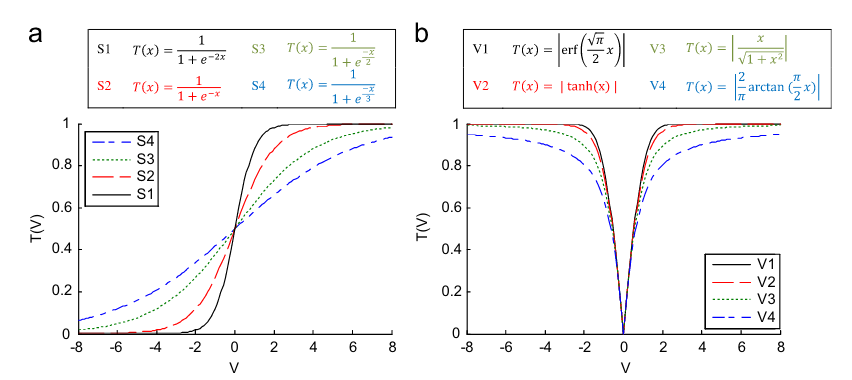
\includegraphics[width=0.8\textwidth]{imagenes/transfer_functions.png}
  \end{center}
  \caption[Funciones de transferencia]{En esta figura extraída de \cite{mirjalili_s-shaped_2013} se muestran funciones del tipo \textbf{S-shaped} (a) y \textbf{V-Shaped} (b).}
\end{figure}